\section{Simulations}\label{sec:simulations}
\hrule

Having developed theoretical results concerning uniform inference methods for the TDNN estimator, we will proceed by testing their properties in several simulation studies.

\subsection{Nonparametric Regression}
To investigate the practicality of the nonparametric regression estimators presented in this paper, we consider a collection of setups.
First, we focus on illustrating the bias correcting properties of the TDNN estimator by replicating some of the findings of \citet{demirkaya_optimal_2024}.
One such promising example is shown in Figure \ref{fig:TDNN_bias_cor} highlighting the potential improvements obtainable by combining multiple subsampling scales.
\begin{figure}[H]
	\centering
	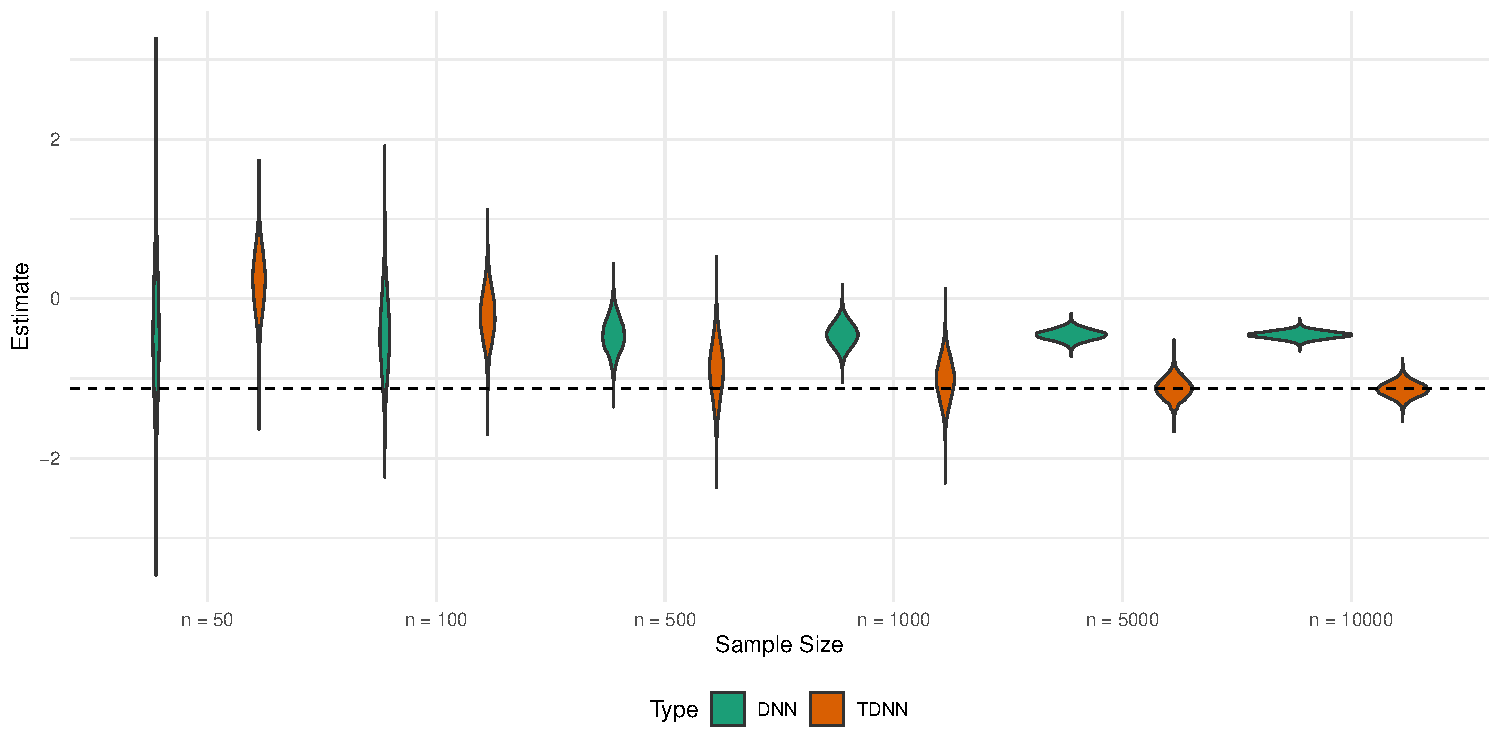
\includegraphics[width = \textwidth]{../Code/Simulations/Graphics/TDNN_DNN.pdf}
	\caption{Comparison of the DNN ($s = 20$) and TDNN ($s_1 = 20, s_2 = 50$) Estimators for different sample sizes.
		The dashed line indicates the value of the unknown regression function at the point of interest.
		Simulation Setup replicates Setting 1 from \citet{demirkaya_optimal_2024} for 10000 Monte Carlo Replications.}
	\label{fig:TDNN_bias_cor}
\end{figure}

As a second, potentially more illustrative example, we consider the estimation of a function of two arguments.
Specifically, we consider the function $\mu(x) = 5 \cdot \left(\cos(x_1) + \cos(x_2)\right)$ on $[0,1]^2$ with heteroskedastic error terms whose variance is determined by $\sigma_{\varepsilon}^2(x) = \frac{1}{100}\left|x_1 + x_2\right|^2$.
The resulting surface is depicted in Figure \ref{fig:reg_surface}.
\begin{figure}[H]
	\centering
	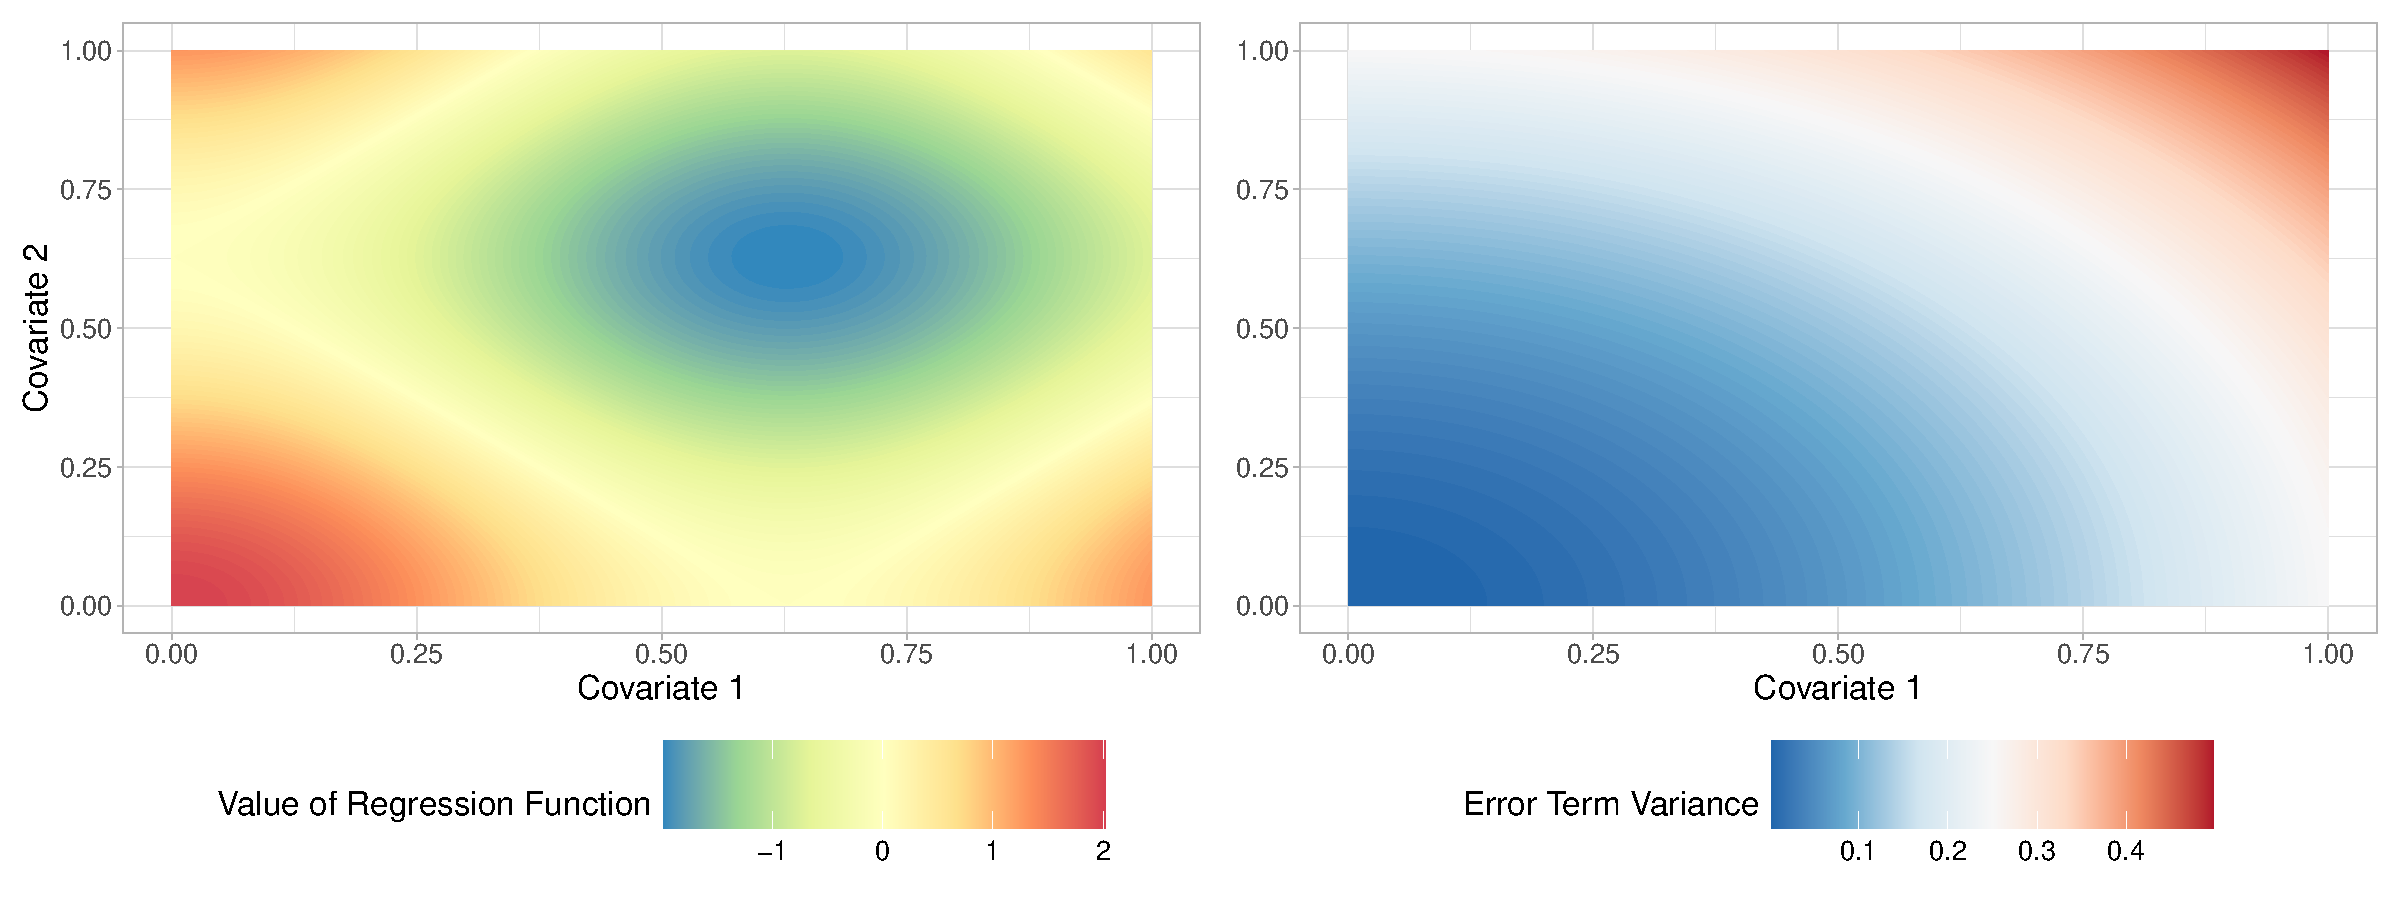
\includegraphics[width = \textwidth]{../Graphics/Reg_Exmp1.pdf}
	\caption{Value of the Regression Function (left) and Variance of the Error Term (right)}
	\label{fig:reg_surface}
\end{figure}

\subsection{CATE-Estimation}

\begin{figure}[H]
	\centering
	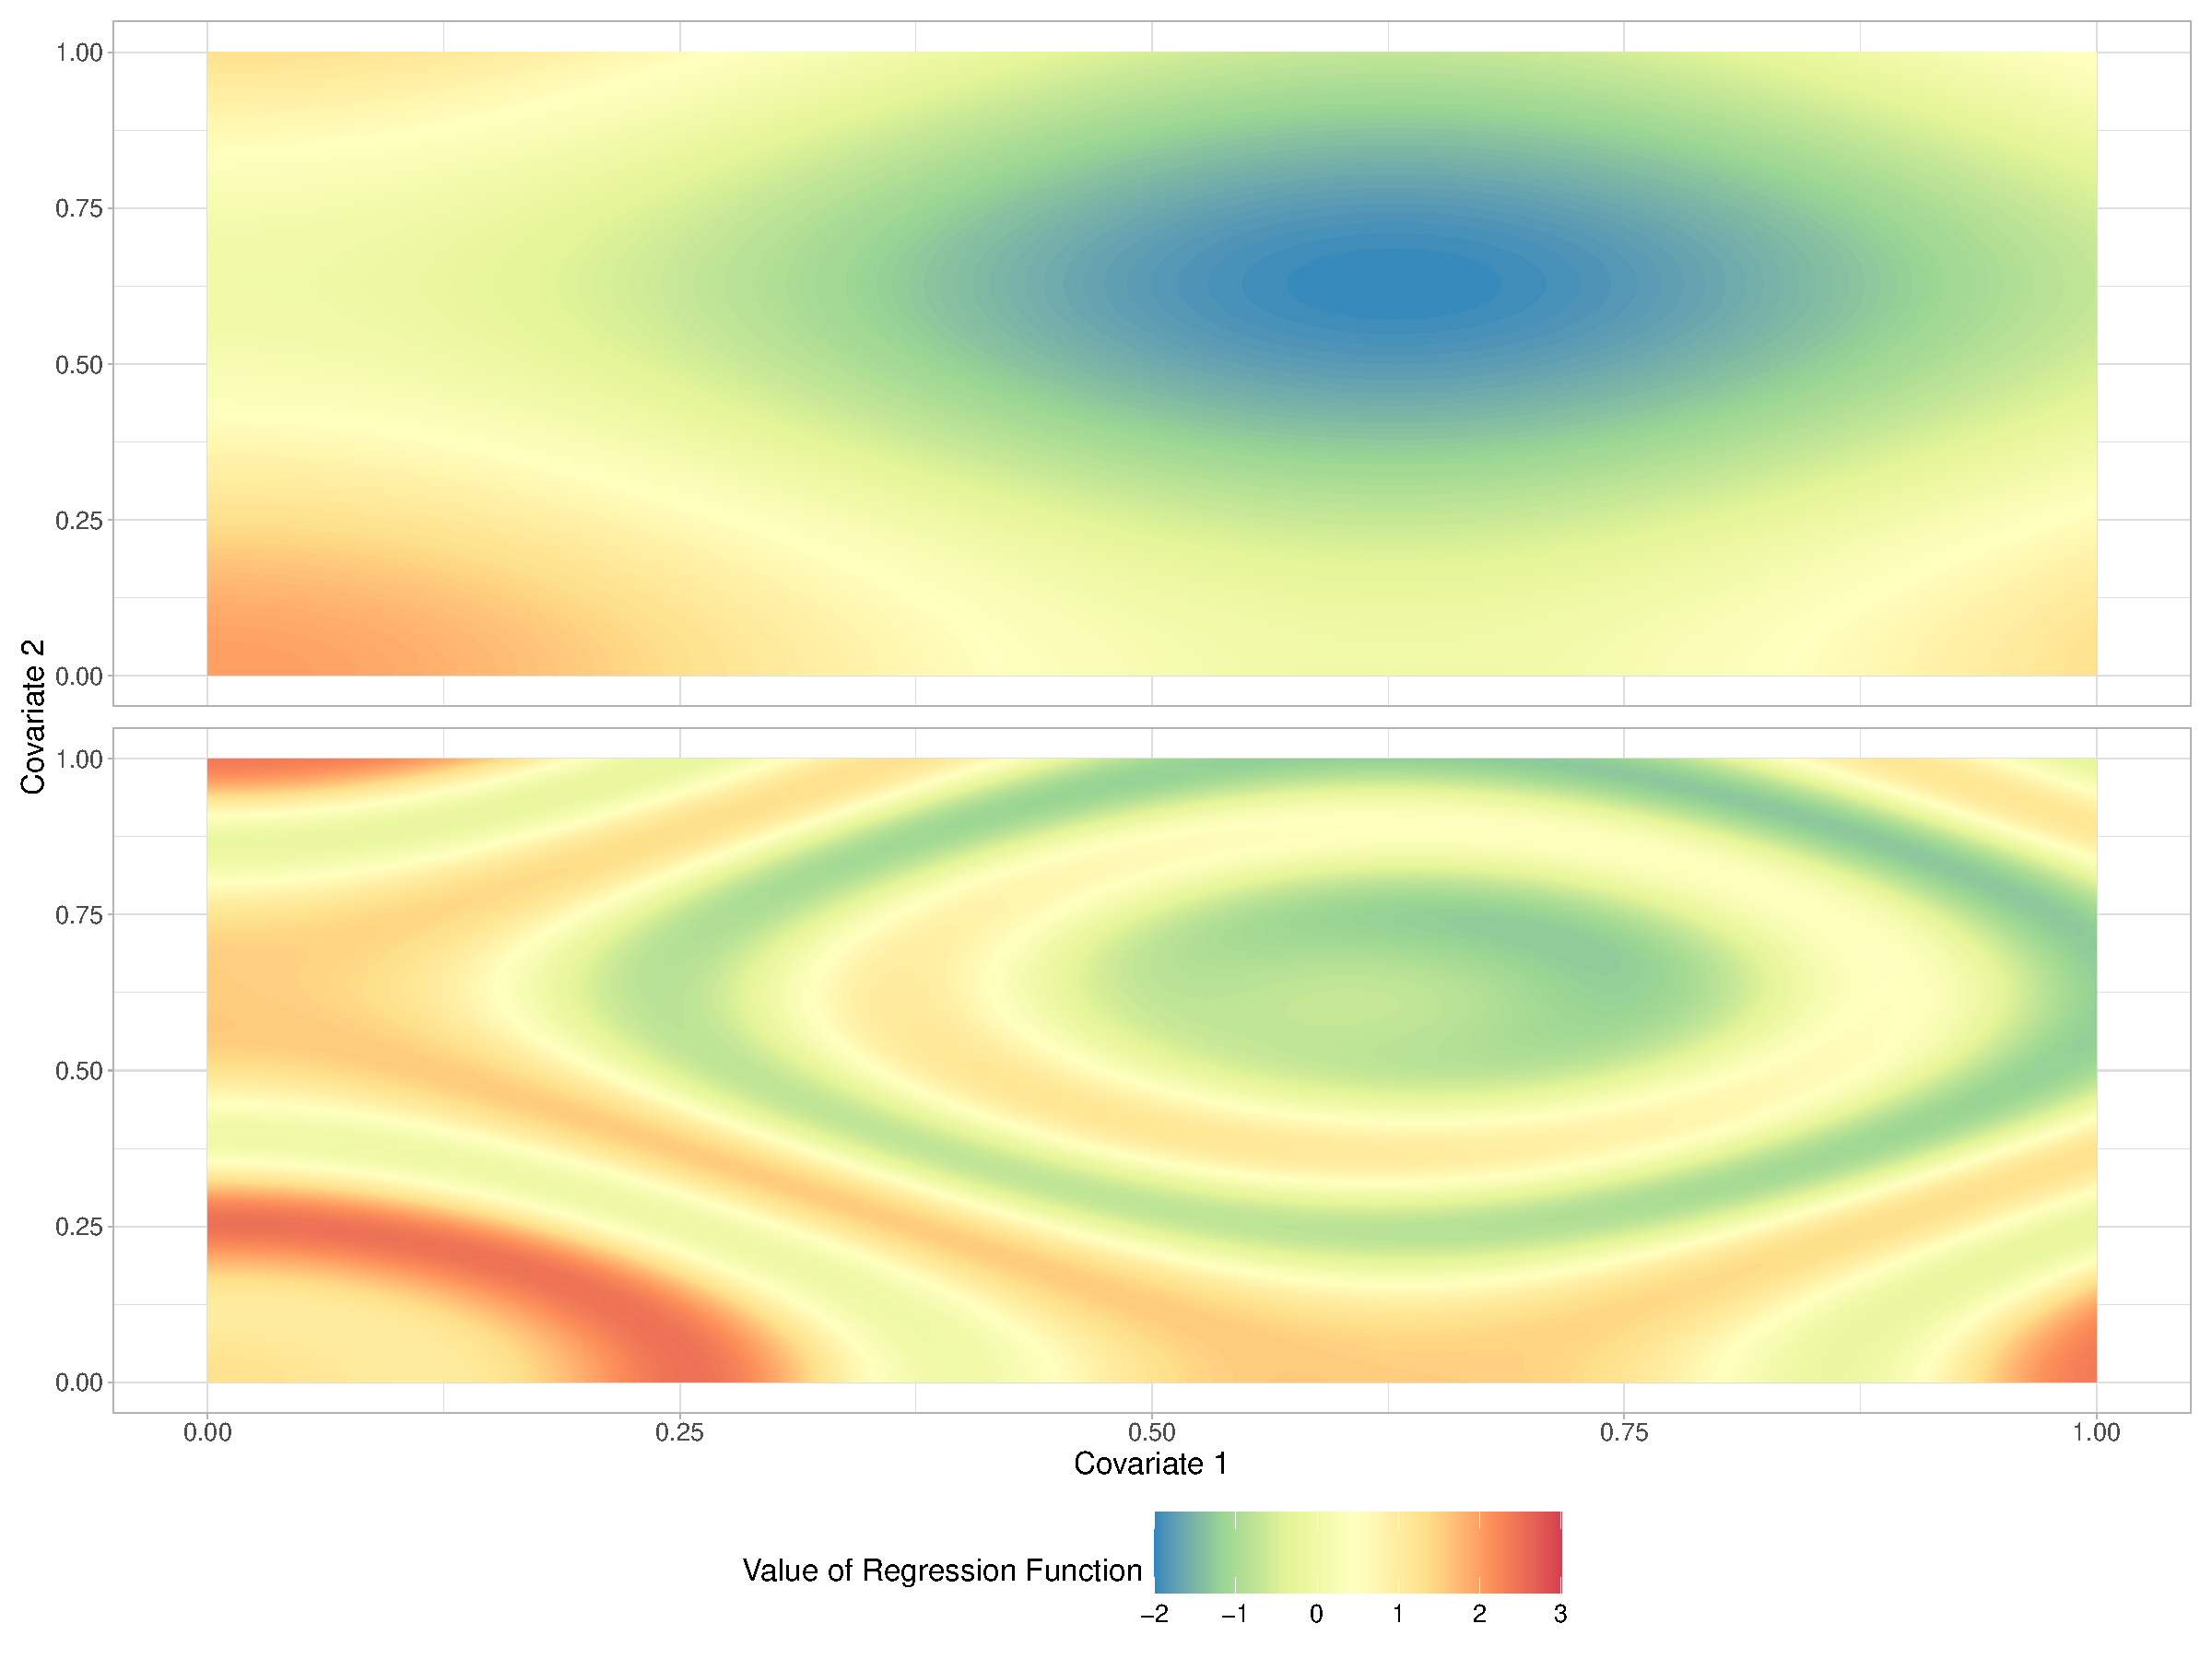
\includegraphics[width = \textwidth]{../Graphics/CATE_Exmp1.pdf}
	\caption{Value of the Regression Functions $\mu_0$ (upper) and $\mu_1$ (lower).	Error term structure remains unchanged.}
	\label{fig:CATE_surfaces}
\end{figure}

{\color{red} LOREM IPSUM}